\documentclass[xcolor=table,10pt,t]{beamer}
\title{CLARIAH Interoperability: FoLiA}
%\subtitle{Text Annotation Formats}
\date{\today}
\author{Maarten van Gompel}
%% Use the official themes as much as possible
%\usetheme[official=false,department=clst]{ruhuisstijl}
%\usetheme[official=false]{ruhuisstijl}
\usetheme[official=true,department=clst]{ruhuisstijl}


\begin{document}

\begin{frame}
    \titlepage{}
        \begin{figure}
        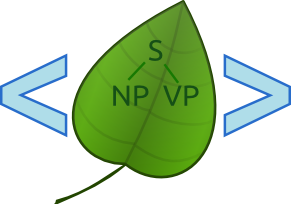
\includegraphics[height=1cm]{../logo.png}
        \end{figure}
        \vspace{3.5cm}
    %\includegraphics[width=5cm]{lama-logo-transparent.png}
\end{frame}

\section{Introduction}

\begin{frame}{Introduction}
    \begin{block}{Introduction}
        FoLiA is a rich XML-based format for linguistic annotation
    \end{block}

	\begin{block}{Intended Applications}
		\begin{itemize}
			\item as a corpus \textbf{storage} format
			\item as a language resource \textbf{exchange} format 
		\end{itemize}				
	\end{block}

    \begin{block}{Aim}
        \begin{itemize}
        \item Provide one solution for a wide variety of linguistic annotation types, using a generic paradigm 
        \item Provide one canonical and validatable serialisation (XML-based)
        \item Provide a \textbf{practical} solution that can be readily adopted
        \begin{itemize}
            \item FoLiA is developed bottom-up alongside tools and libraries and extended as needed
        \end{itemize}
        \end{itemize}
    \end{block}
\end{frame}

\section{Characteristics}

\begin{frame}{Characteristics (1/3)}
    \begin{block}{FoLiA Paradigm}
        \textbf{Consistent} and \textbf{generic} framework accross various linguistic annotation types.
        \begin{itemize}
            \item \textbf{Separation of label semantics} from the format itself. FoLiA does not
                commit to any label set or language. Label sets are defined in
                separate \emph{set definitions}. Annotations carry
                \emph{classes} that are defined by these sets.
            \item \textbf{Specific} -- Various specific annotation types are defined.
            \item \textbf{Expressive} -- Verbose expression of annotations:
                globally unique identifiers, their annotators, timestamps, confidence values, etc... Support for
                \emph{alternative} annotations, corrections of any annotation.
            \item \textbf{Formalised} -- Validation on shallow (structural) or
                deep level. 
        \end{itemize}
    \end{block}
\end{frame}

\begin{frame}{Characteristics (2/3)}
    \begin{block}{FoLiA Format}
        \begin{itemize}
            \item \textbf{Document-based} -- One document, one XML file
            \item Retains \textbf{structural} information (like TEI, but not as expressive), \textbf{integrated} approach.
            \item \textbf{Localised} -- Annotations are stored in close proximity to the textual items they describe. This facilitates streaming parsers.
        \end{itemize}
    \end{block}
\end{frame}

\begin{frame}{Characteristics (3/3)}
    \begin{block}{Annotation types}
        Annotation types can be grouped as follows:
        \begin{itemize}
            \item \textbf{Structural Annotation} -- Annotation of document structure: divisions, paragraphs, sentences, words/tokens, lists, tables, etc..
            \item \textbf{Token Annotation} -- Annotation pertaining to a token (or other structural element): part-of-speech, lemmas, lexical semantic senses
            \item \textbf{Span Annotation} -- Annotation spanning multiple tokens: (named) entities, dependency relations, semantic roles, coreference relations, syntactic parsers
            \item \textbf{Higher-order annotations} -- Annotations on annotations: corrections, alternatives, comments, descriptions, references to internal or external sources (alignments), annotation of arbitrary substrings
        \end{itemize}
    \end{block}
\end{frame}


\section{Context}

\begin{frame}{Context: Metadata}
  \begin{block}{Metadata}
        Documents can ...
        \begin{itemize}
            \item ...refer to external metadata files (any format)
            \item ...embed other XML-based metadata schemes (e.g.  CMDI, Dublin Core)
            \item ...use FoLiA's native metadata scheme (a simple key value store)
        \end{itemize}
  \end{block}
\end{frame}


\begin{frame}{Context: Set Definitions}
  \begin{block}{Set definitions}
        \begin{itemize}
            \item Documents declare what annotation types they make use of and
                what sets are used.
            \item ...declarations refer to external set definition files
            \item A set definition defines what classes are part of a
                particular label set.
            \item ... classes may be linked to data category
                registries/ontologies for formal semantic closure.
            \item Annotations refer to classes
        \end{itemize}

        \begin{itemize}
            \item Set definitions are currently expressed in a simple XML
                format
            \item Considering moving these to RDF
        \end{itemize}
  \end{block}
\end{frame}


\begin{frame}{Context: Converters (1/2)}
  \begin{block}{Converters: To FoLiA from ...}
      \begin{itemize}
          \item Alpino XML
          \item ALTO XML (OCR output)
          \item DCOI (legacy)
          \item HTML (via INL's \emph{OpenConvert}, limited)
          \item HOCR (HTML OCR output from \emph{Tesseract})
          \item NAF (work-in-progress)
          \item plain text (via tokeniser \emph{ucto} or
              \emph{OpenConvert} (INL))
          \item Political Mashup XML
          \item ReStructuredText
          \item TEI (via INL's \emph{OpenConvert}, limited)
          \item MS Word (via INL's \emph{OpenConvert}, limited)
      \end{itemize}
  \end{block}
\end{frame}


\begin{frame}{Context: Converters (2/2)}
  \begin{block}{Converters: From FoLiA to ...}
      \begin{itemize}
          \item DCOI
          \item HTML (for rich visualization)
          \item NAF (work-in-progress, by Antske)
          \item plain text
          \item plain text enriched with token annotations (limited)
          \item simple columned format (one token per line, limited)
          \item ReStructuredText
          \item TEI (via INL's \emph{OpenConvert}, limited)
      \end{itemize}
  \end{block}
\end{frame}

\begin{frame}{Context: Software Libraries}
    \begin{block}{Software Libraries}
      \begin{itemize}
        \item for Python: part of \emph{PyNLPl}
        \item for C++: \emph{libfolia} (by Ko van der Sloot, RU)
      \end{itemize}
    \end{block}
\end{frame}

\begin{frame}{Context: Utilities}
    \begin{block}{Utility collections}
      \begin{itemize}
          \item foliatools (python based)
          \item foliautils (c++ based)
      \end{itemize}
    \end{block}
    \begin{block}{Utilities (CLI)}
      \begin{itemize}
          \item \textbf{foliavalidator} or \textbf{folialint} - FoLiA validators
          \item foliacorrect (tool to deal with corrections in FoLiA)
          \item foliacount (compute simple statistics)
          \item folia-idf (IDF statistics for a directory of FoLiA documents)
          \item folia-langcat (language detection)
          \item foliamerge (merge multiple folia documents)
          \item foliaquery (query FoLiA documents, using FQL or CQL) 
          \item foliacorrect (tool to deal with corrections in FoLiA)
          \item various of the earlier mentioned converters
      \end{itemize}
    \end{block}
\end{frame}


\begin{frame}{Context: FoLiA-aware Software (1/3)}
    \begin{block}{FoLiA-aware NLP Software}
      \begin{itemize}
        \item \textbf{ucto} - Tokeniser, multilingual, can read and produce FoLiA
        \item \textbf{Frog} - NLP Suite for dutch: tokenisation (via ucto),
            PoS-tagging, lemmatisation, morphological analysis, shallow
            parsing, named entity recognition, dependency parsing. Can read and
            output FoLiA.
        \item \textbf{Gecco} - Generic Environment for Context-aware Correction of
            Orthography: spelling correction software, backend for
            \textbf{Valkuil.net}. Outputs FoLiA.
        \item \textbf{TICCL} - Text-induced Corpus Cleanup: Text normalisation
            and post-OCR correction system. Outputs FoLiA.
        \item \textbf{Colibri Core} - Pattern counting and extraction, limited
            FoLiA input support
      \end{itemize}
    \end{block}
\end{frame}


\begin{frame}{Context: FoLiA-aware Software (2/3)}
    \begin{block}{Search software}
      \begin{itemize}
        \item \textbf{BlackLab} - Corpus retrieval engine with (limited) indexing support for FoLiA (INL)
        \item \textbf{WhiteLab} - Web application for the search and
            exploration of large corpora with linguistic annotations (Matje van de Camp, TaalMonsters)
        \item \textbf{PaQu} - Parse and search in syntactically annotated
            corpora (Groningen University)
      \end{itemize}
    \end{block}
\end{frame}

\begin{frame}{Context: Folia-aware Software (3/3)}
    \begin{block}{FLAT (FoLiA Linguistic Annotation Tool)}
      \begin{itemize}
            \item A web-based collaborative annotation tool
            \item Eventually aims to support annotation for all annotation
                types supported in FoLiA.
            \item Used for multiple projects; recently adopted by PARSEME for annotation of MWEs as well
            \item backend: FoLiA Document Server (\emph{foliadocserve})
            \item communication: \textbf{FoLiA Query Language (FQL)}
            \item Public installation: \url{http://flat.science.ru.nl}
      \end{itemize}
    \end{block}
\end{frame}

\begin{frame}{Context: Folia-aware Software (3/3)}
        \includegraphics[width=115.0mm]{/home/proycon/work/flat/docs/ner.png}
\end{frame}

\section{Discussion}

\begin{frame}{Discussion: Interoperability}
    \begin{block}{Aims for the future}
        \begin{itemize}
            \item Continued work to extend the format and libraries on a need-to basis
            \item Continued support to all parties using FoLiA
            \item Continued work on FLAT
            \item Finish the FoLiA/NAF conversion tools
            \item More converters? If so, which?
            \item Migrate set definitions to RDF?
            \item What is the desireability of more RDF support? I.e. RDF
                schema for FoLiA and conversion to RDF for annotated documents.  Use cases?
        \end{itemize}
    \end{block}
\end{frame}

\begin{frame}{Discussion: Questions?}
        \vspace{3.5cm}
        \begin{figure}
        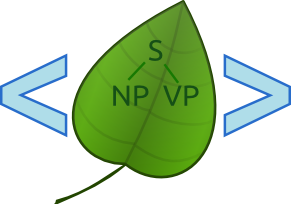
\includegraphics[height=1cm]{../logo.png}
        \end{figure}
\end{frame}


\end{document}
